\documentclass[fullapage,12pt]{article}
\usepackage{fancybox}
\usepackage{graphicx}
\usepackage{amssymb}
\usepackage{amsmath}
\usepackage{epsfig}
\usepackage{color}
\usepackage{multicol}
\usepackage{hhline}
\usepackage{xspace,epic,eepic,graphicx}
\usepackage{latexsym}
\usepackage{enumerate}

\newcommand{\mc}[1]{\mathcal{ #1}}
\newcommand{\e}[1]{\emph{#1}}
\newcommand{\ignore}[1]{}
\newcommand{\boxtheorem}{\hfill $\Box$\\}
\newcommand{\nit}[1]{{\it #1}}



\begin{document}
\thispagestyle{empty}

\vspace*{-3.5cm}
\begin{center} \bf \large COMP 3400~ Computational Logic and Automated Reasoning\\ Winter 2017~~ Assignment 3
\end{center}

{\small \noindent {\bf Instructions:}
\begin{enumerate}
\item {\bf \Large For your solution use the template file that was posted on the course news, and follow the instructions in it.}

In particular: (a) Include at the top of the first page: full name, student number, and email address.
(b) {\bf Assignments have to be created with Latex, and submitted in pdf format, as a single file}. (c) Every problem solution MUST include
the problem statement, even if the assignment does not (sometimes the assignments will refer to slides presented in class). The source file for this assignment is provided.

Latex has to be used as such, not as you would use a text editor, such as Notepad. In particular,  formulas have to be written using Latex's mathematical
features, and then compiled.

\item Assignments are individual, no groups.
\item  %Use the same format as this document (the Latex source is provided with the pdf).
Submit by email to the instructor, with ``Assignment "Number", CompLog" in the subject. {\bf Include your last name in the file name!} For example,
in the subject: \ ``Assig. 3 CompLog". The file name: \ ``YourLastName-3.pdf".

{\bf Only a single pdf file will be accepted as submission (nothing other than a pdf file will be accepted). No tar or zip files (or anything like that), please. Keep your Latex source files in case you are requested to show them.}

\item Explain your solution very carefully, but still be succinct with your answers. No unnecessary verbose arguments, please. Go to the point.

Make explicit all your assumptions.

\item {\bf Not following the instructions above or the solution template file will make you lose points.}
\end{enumerate}}


\noindent 1. \ A binary adder is shown in Figure \ref{fig:adderNoNums}. The adder, on test inputs may be showing
unintended  results. Actually, the input values are:
\ $A=0, \ B=1,\ C=0$; and the output values are: $D=0 \ E=1$.\\
\\
(a) Outside Prover9 (using formulas written with Latex), construct a weak-failure model of the circuit using {\bf PROPOSITIONAL LOGIC}.
\ {\bf Explain each formula and its role in the model. Start by listing the propositional variables and their intended meanings.}\\
\\
(b) You want to obtain minimal {\em conflicts}, that is, sets of components that cannot be all simultaneously working
 well  at the light of the observation. \ (Minimality means in this case that no proper
subset of a conflict is a conflict.)

Before going into Prover9, explain your methodology based on automated reasoning \`a la Prover9 for obtaining: (a) conflicts, (b) minimal ones (how can you be sure?), and (c) more than one with the same general specification.
\\
\\
(c) Use Prover9 to obtain all possible minimal conflicts. Show the main ingredients of the input file, with an
explanation. Do the same with the output file, interpreting and explaining the results.\\
\\
(d)  Attach as appendices the full input and output files (including the runs) for the parts above, clearly indicating each of them. \\



%\vspace*{-3cm}
\begin{figure}[h]
\begin{center}
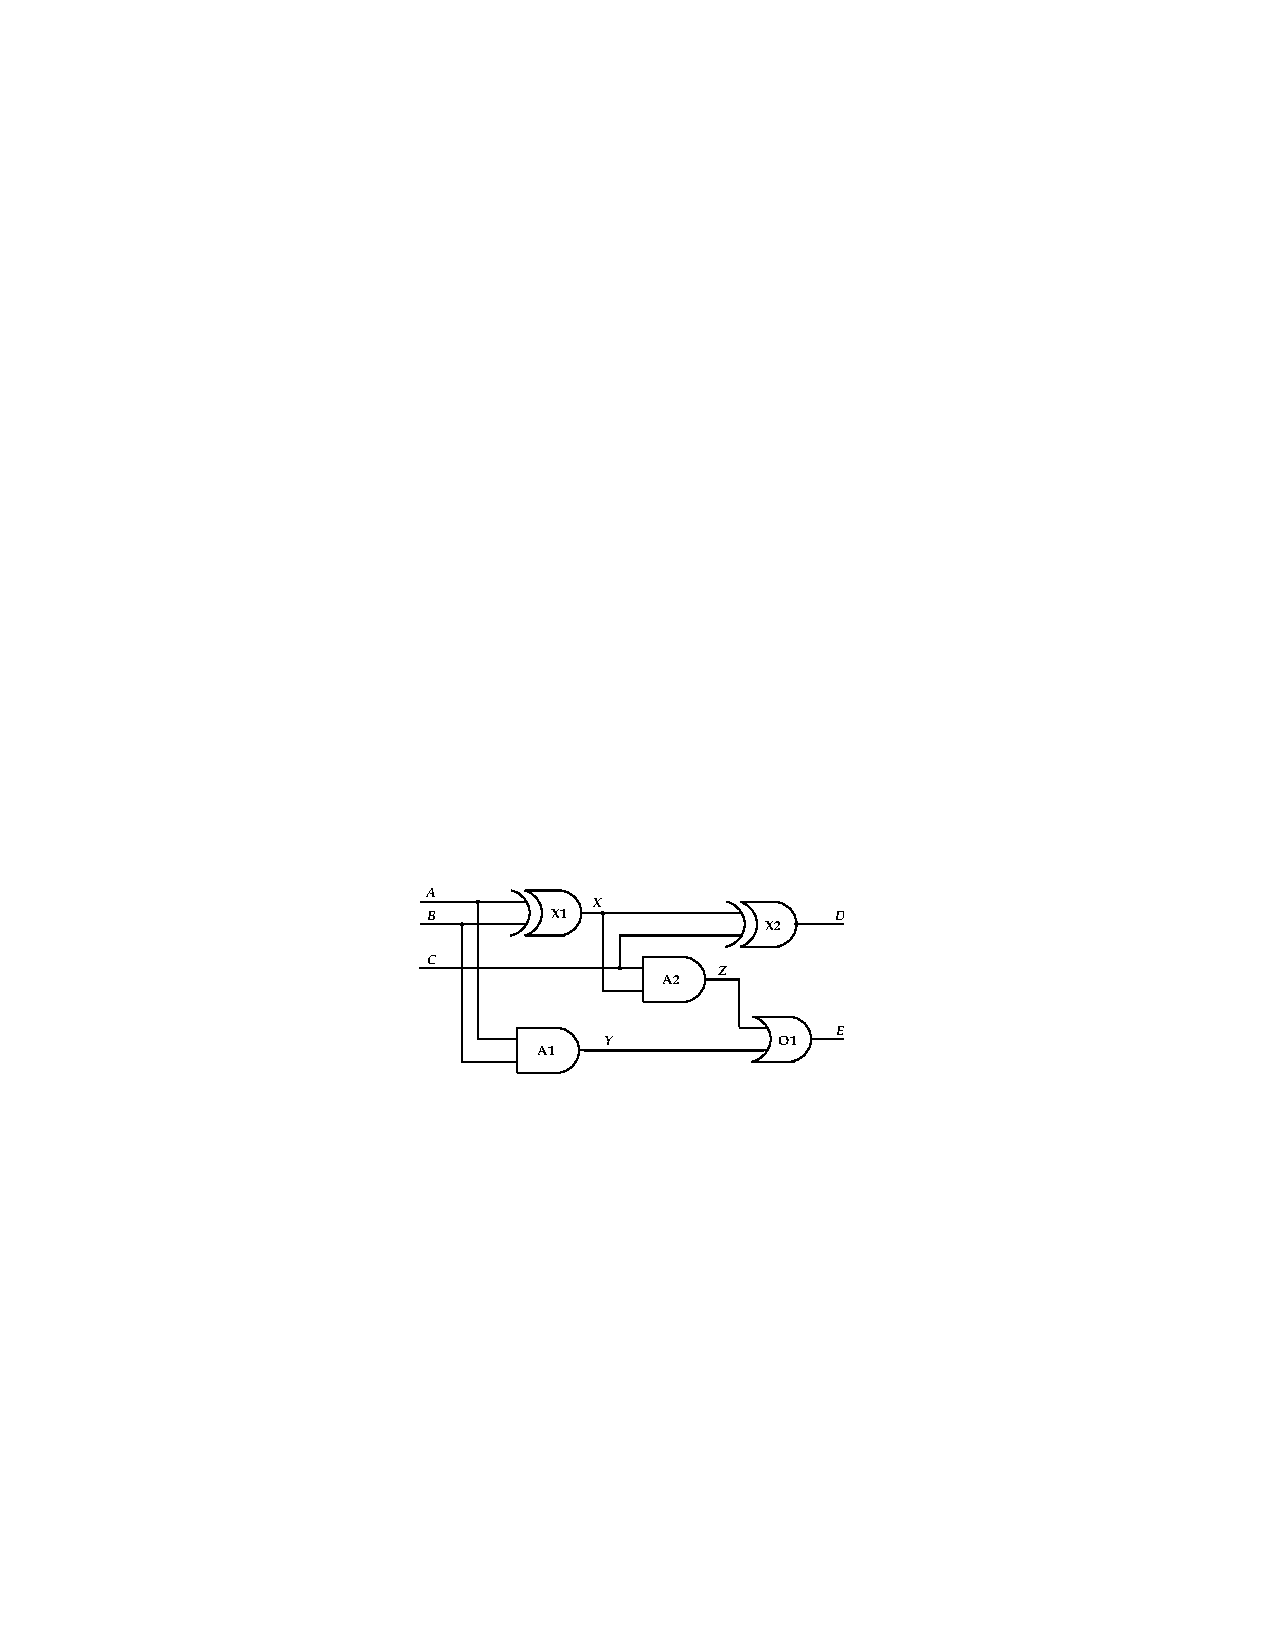
\includegraphics[width=7cm]{adderNoNums.pdf}
\caption{A Complete Adder}\label{fig:adderNoNums}
\end{center}
\end{figure}
\vspace{-5mm}(Gates {\tt X1}, {\tt X2} are exclusive or-gates)\\

\noindent 2. \ (a) Produce a knowledge base (program) in {\bf PROPOSITIONAL PROLOG} capturing the following information as closely as possible as stated here: {\em If Tweety is a bird and it is not an abnormal bird, then it flies. \
A bird is abnormal exactly when it is an ostrich, a penguin, or not an abnormal wooden bird. A wooden bird is abnormal exactly when operated under remote control. Tweety is a bird, it is  not
an ostrich nor a penguin nor a remote controlled wooden bird.}  \ {\bf All this has to be provided as a set of clauses (rules) outside Prolog, using formulas written in Latex. Start by listing the propositional variables and their intended meanings.} Notice that the two forms of abnormality mentioned here may be different, one is if birds, the other is for wooden birds.\\
\\
(b) Show by means of a refutation tree developed \'a la Prolog that  {\em Tweety flies} \ (as we did in class).\\
\\
(c) Now use SWI Prolog to prove that {\em Tweety flies}. Explain your approach and what Prolog shows through its run. Attach a file showing the input file, and the whole run (interaction, trace) with Prolog.  \\




{\bf The whole assignment has to be submitted as a single PDF file.}

\noindent {\bf Deadline: \ March 6, at 23:55}




\end{document}
